\documentclass[12pt, a4paper]{report}
\usepackage[portuguese]{babel}
\usepackage{graphicx} 
\usepackage{setspace}

\title{Algoritmos Para Achar Raízes Reais de Polinômios}
\author{Eros Moreira Ferreira}
\date{May 2024}

\begin{document}

\maketitle

\section{Introdução}

Diversos problemas exigem cálculos do tipo $f(x) = 0$, que usualmente são resolvidas de maneira simbólica. Porém, algumas soluções simbólicas são extremamente complicadas, e aproximações numéricas se tornam necessárias.

Como exemplo, resolvemos uma equação do tipo $P(x)-Q(x) = 0$, ou seja, a interseção entre funções.
As funções utilizadas são
\begin{displaymath}
    P(x) = xtanx \hspace{1cm}  Q(x) = \sqrt{16-x^2}
\end{displaymath}
definidas para $x>0$ e tal que $P(x)>0$, $Q(x)>0$.

Ao plotar das duas equações vemos que existem 2 pontos de interseção, que ocorrem no intervalo $1.0<x<1.5$ e $3.0<x<4.0$.

\begin{figure}[h]
    \centering
    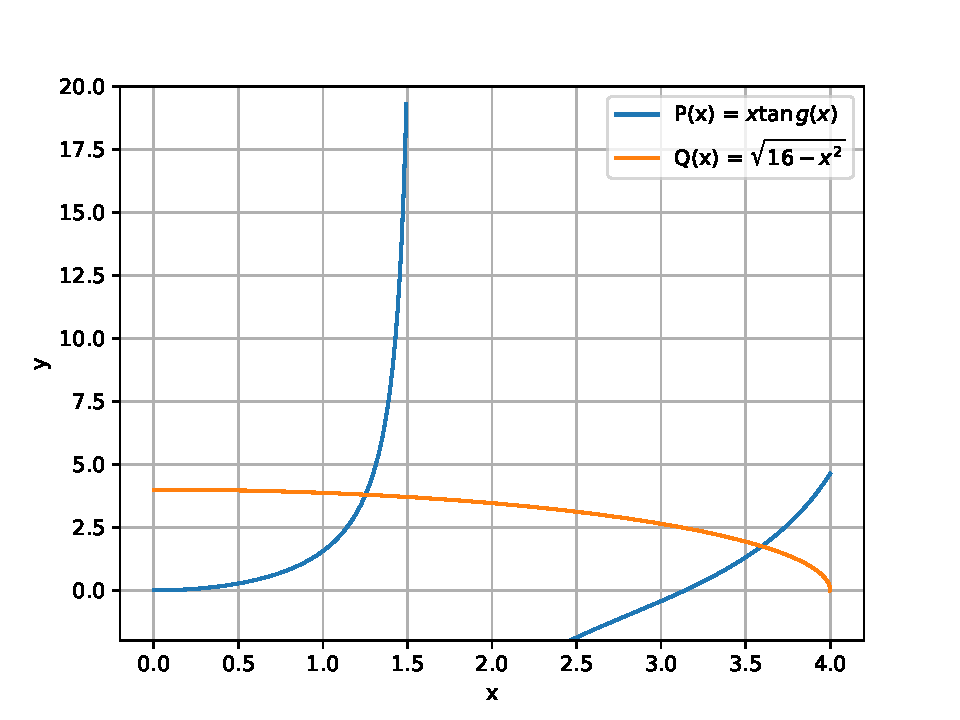
\includegraphics[width=0.8\linewidth]{bissecao.pdf}
    \caption{Interseção entre P(x) e Q(x)}
    \label{fig:enter-label}
\end{figure}

Esses intervalos serão utilizados pelos dois métodos empregados para achar raízes reais da função $f(x) = P(x)-Q(x)$.

\section{Método da Bisseção}

Esse método consiste na escolha de dois pontos iniciais $a_0$ e $b_0$, com $a_0 < b_0$, de modo que $f(a_0)f(b_0)<0$. O teorema do valor intermediário garante que existe uma raiz no intervalo $[a,b]$ se a função $f(x)$ é contínua nesse intervalo. Escolhido os pontos iniciais, o método segue os seguintes passos:

\begin{itemize}
    \item \textbf{Passo 1:} A aproximação para a raiz será $x_0 = \frac{a_0+b_0}{2}$.
    
    \item \textbf{Passo 2:} Verificar se $x_0$ atende o critério de parada, que pode ser o erro entre iterações sucessivas $|x_k - x_{k-1}|$ ou o erro relativo entre iterações sucessivas $\frac{|x_k - x_{k-1}|}{|x_k|}$ (assumindo $x_k \neq 0$), ou ainda verificar se $|f(x_k)|$ é pequeno.

    \item \textbf{Passo 3:} Se não atende o critério de parada, o novo intervalo será $x_0 = a_1$ e $b_1 = b_0$ se $f(x_0)f(b_0)<0$, ou $x_0 = b_1$ e $a_1 = a_0$ caso ao contrário.
    
    \item \textbf{Passo 4:} Repetir até o critério de parada ser satisfeito.
\end{itemize}

Esse método sempre converge para uma solução se o critério de escolha dos pontos for atendido.

\section{Método de Newton-Raphson}

\begin{itemize}
    \item \textbf{Passo 0:} Escolhe-se um ponto inicial $x_0$, de modo que $\frac{d(x_0)}{dx} \neq 0$, que seja próximo da raiz desejada.

    \item \textbf{Passo 1:} Calcule a equação da reta tangente nesse ponto. O ponto $x_1$ que essa reta corta o eixo $X$ será a nova aproximação da raiz.

    \item \textbf{Passo 2:} Verificar se $x_1$ atende o critério de parada, que pode ser o erro entre iterações sucessivas $|x_k - x_{k-1}|$ ou o erro relativo entre iterações sucessivas $\frac{|x_k - x_{k-1}|}{|x_k|}$ (assumindo $x_k \neq 0$), ou ainda verificar se $|f(x_k)|$ é pequeno.

    \item \textbf{Passo 3:} Caso não atenda o critério, $x_0 = x_1$ e se repete o passo 1 e 2 até $x_k$ atender o critério de parada. 

\end{itemize}
 
\section{Resultados}
No método da bisseção foi utilizado como critério de parada $|x_k - x_{k-1}| < \epsilon$, sendo $\epsilon = 10^{-5}$.
Os pontos utilizados foram $a_0 = 1$ e $b_0 = 1.5$ para a $raiz_1$, $a_0 = 3.5$ e $b_0 = 4$ para a $raiz_2$.

No método de Newton-Raphson foi utilizado o mesmo critério de parada. Os pontos foram $x_0 = 1.5$ e $x_0 = 3.5$ para a $raiz_1$ e $raiz_2$ respectivamente.

Os resultados para o método da bisseção foram:
\begin{displaymath}
    raiz_1 = 1.25236 \hspace{1cm} raiz_2 = 3.59530
\end{displaymath}
com 16 interações ambas.

Para o método de Newton-Raphson:
\begin{displaymath}
    raiz_1 = 1.25235 \hspace{1cm} raiz_2 = 3.59530
\end{displaymath}
com 6 e 3 iterações respectivamente.

O método de Newton-Raphson convergiu mais rápido para as raízes, o que é esperado já que possui ordem de convergência quadrática. Já o método da bisseção possui ordem de convergência linear, tendendo a demorar mais para convergir.

Houve uma diferença no último dígito da $raiz_1$, o que é explicado pelo fato da precisão ser de 5 casas decimais, o último é duvidoso.
\end{document}
